\subsection{Metodología de Calibración}

El ajuste del instrumento virtual se llevó a cabo mediante un procedimiento de calibración lineal de dos puntos. Este proceso permitió corregir los errores sistemáticos de la etapa de acondicionamiento analógico y establecer la trazabilidad de las medidas.

\begin{enumerate}
    \item \textbf{Fijación del Cero Metrológico (\textit{Tara}):} Con el sistema mecánico en reposo y la plataforma de pesaje completamente vacía, se procedió a la captura de la tensión residual. Esta medición en crudo absorbe el desequilibrio estático del puente de Wheatstone, las tensiones de \textit{offset} del amplificador de instrumentación AD623 y el pedestal de referencia de 1.607~voltios. El algoritmo en \textit{LabVIEW} almacena este valor como el cero del sistema, restándolo de forma sistemática en las lecturas subsecuentes.
    
    \item \textbf{Ajuste del \textit{Span} (Pendiente):} Posteriormente, se aplicó sobre la célula de carga una masa de referencia aproximado de 1.000~kg, empleado como peso patrón. Al estabilizarse la señal, el \textit{software} registró la tensión neta correspondiente al fondo de escala operativo y calculó de forma automática el factor de ganancia global (pendiente de la recta de calibración).
\end{enumerate}

La sensibilidad empírica resultante del proceso de calibración arrojó un valor de 642.49~\si{\frac{V}{g}}.

Este valor se calculó teóricamente de la siguiente manera, se tomaron dos medidas:

\begin{itemize}
    \item $V_{diff}$ (sin carga): -1.17588 \si{V}
    \item $V_{diff}$ (con carga de 1 \si{kg}): 0.378307 \si{V}
\end{itemize}

Hallamos la sensibilidad del sistema con esos valores: 

\begin{itemize}
    \item Sensibilidad en \si{\frac{V}{g}}
    $S=\frac{0.378307 - (-1.17588)}{1000} = 0.001554 $ \si{\frac{V}{g}}
    \item Sensibilidad en \si{\frac{g}{V}}
    $S=\frac{1000}{0.378307 - (-1.17588)} = 643.42 $ \si{\frac{g}{V}}
\end{itemize}



\subsection{Análisis de Desempeño y Caracterización Metrológica}

Para evaluar de manera crítica el comportamiento dinámico y estático del sistema, se realizó una caracterización completa que abarca el rango dinámico, la linealidad y la estabilidad temporal de la lectura.

\subsubsection{Contraste Empírico sin Carga}
Antes de la supresión por \textit{software} mediante la tara, se midió físicamente la tensión sin carga directamente a la salida del amplificador de instrumentación, registrándose un valor experimental de [COMPLETAR]~V. Este resultado se contrastó con el límite teórico de seguridad calculado en el análisis de tolerancias (\textit{Worst-Case DC}) de la sección 2. Dado que el valor experimental se encuentra notablemente por debajo del umbral de saturación previsto en el peor escenario de polaridad, se demuestra matemáticamente la validez del pedestal de referencia de 1.607~V introducido para evitar el corte en el canal de adquisición.

\subsubsection{Linealidad y Rango Dinámico}
El rango dinámico verificado de la báscula se extiende desde los 0~g hasta un límite superior de carga de 5~kg, asegurando márgenes de seguridad frente a la saturación del ADC de la tarjeta de adquisición de datos (DAQ).

El error de linealidad máximo registrado fue de [COMPLETAR]~g, confirmando un comportamiento altamente lineal en todo el rango de operación debido a la simetría simétrica de la red de filtros analógicos y al equilibrio de impedancias preservado.

\subsubsection{Estabilidad de la Lectura y Resolución Efectiva}
El impacto del promediado estadístico implementado en el instrumento virtual se demostró empíricamente al contrastar la señal en crudo frente a la señal filtrada.

Tras activar la ventana de promediado por bloques de 32 muestras en \textit{LabVIEW}, se logró una disminución  de las fluctuaciones de alta frecuencia, demostrando una mejora en la resolución efectiva del sistema sin comprometer el tiempo de respuesta demandado para el pesaje estático.

\subsection{Montaje Físico y Disposición Mecánica}

El montaje físico final se muestra en la figura \ref{fig:montaje_hardware} muestra la implementación de la etapa analógica en la placa de pruebas, caracterizada por un ruteado simétrico para proteger el CMRR. Por otro lado, la figura \ref{fig:celda_carga} ilustra la disposición mecánica de la célula de carga acoplada a la estructura rígida de soporte.

\begin{figure}[H]
    \centering
    \includegraphics[width=0.8\linewidth]{figs/montaje_hardware.png}
    \caption{Montaje físico real de la etapa de acondicionamiento eléctrico en la placa de pruebas.}
    \label{fig:montaje_hardware}
\end{figure}


\begin{figure}[H]
    \centering
    \includegraphics[width=0.8\linewidth]{figs/celda_carga.png}
    \caption{Disposición mecánica de la célula de carga y su acoplamiento estructural para el pesaje.}
    \label{fig:celda_carga}
\end{figure}



\begin{figure}[H]
    \centering
    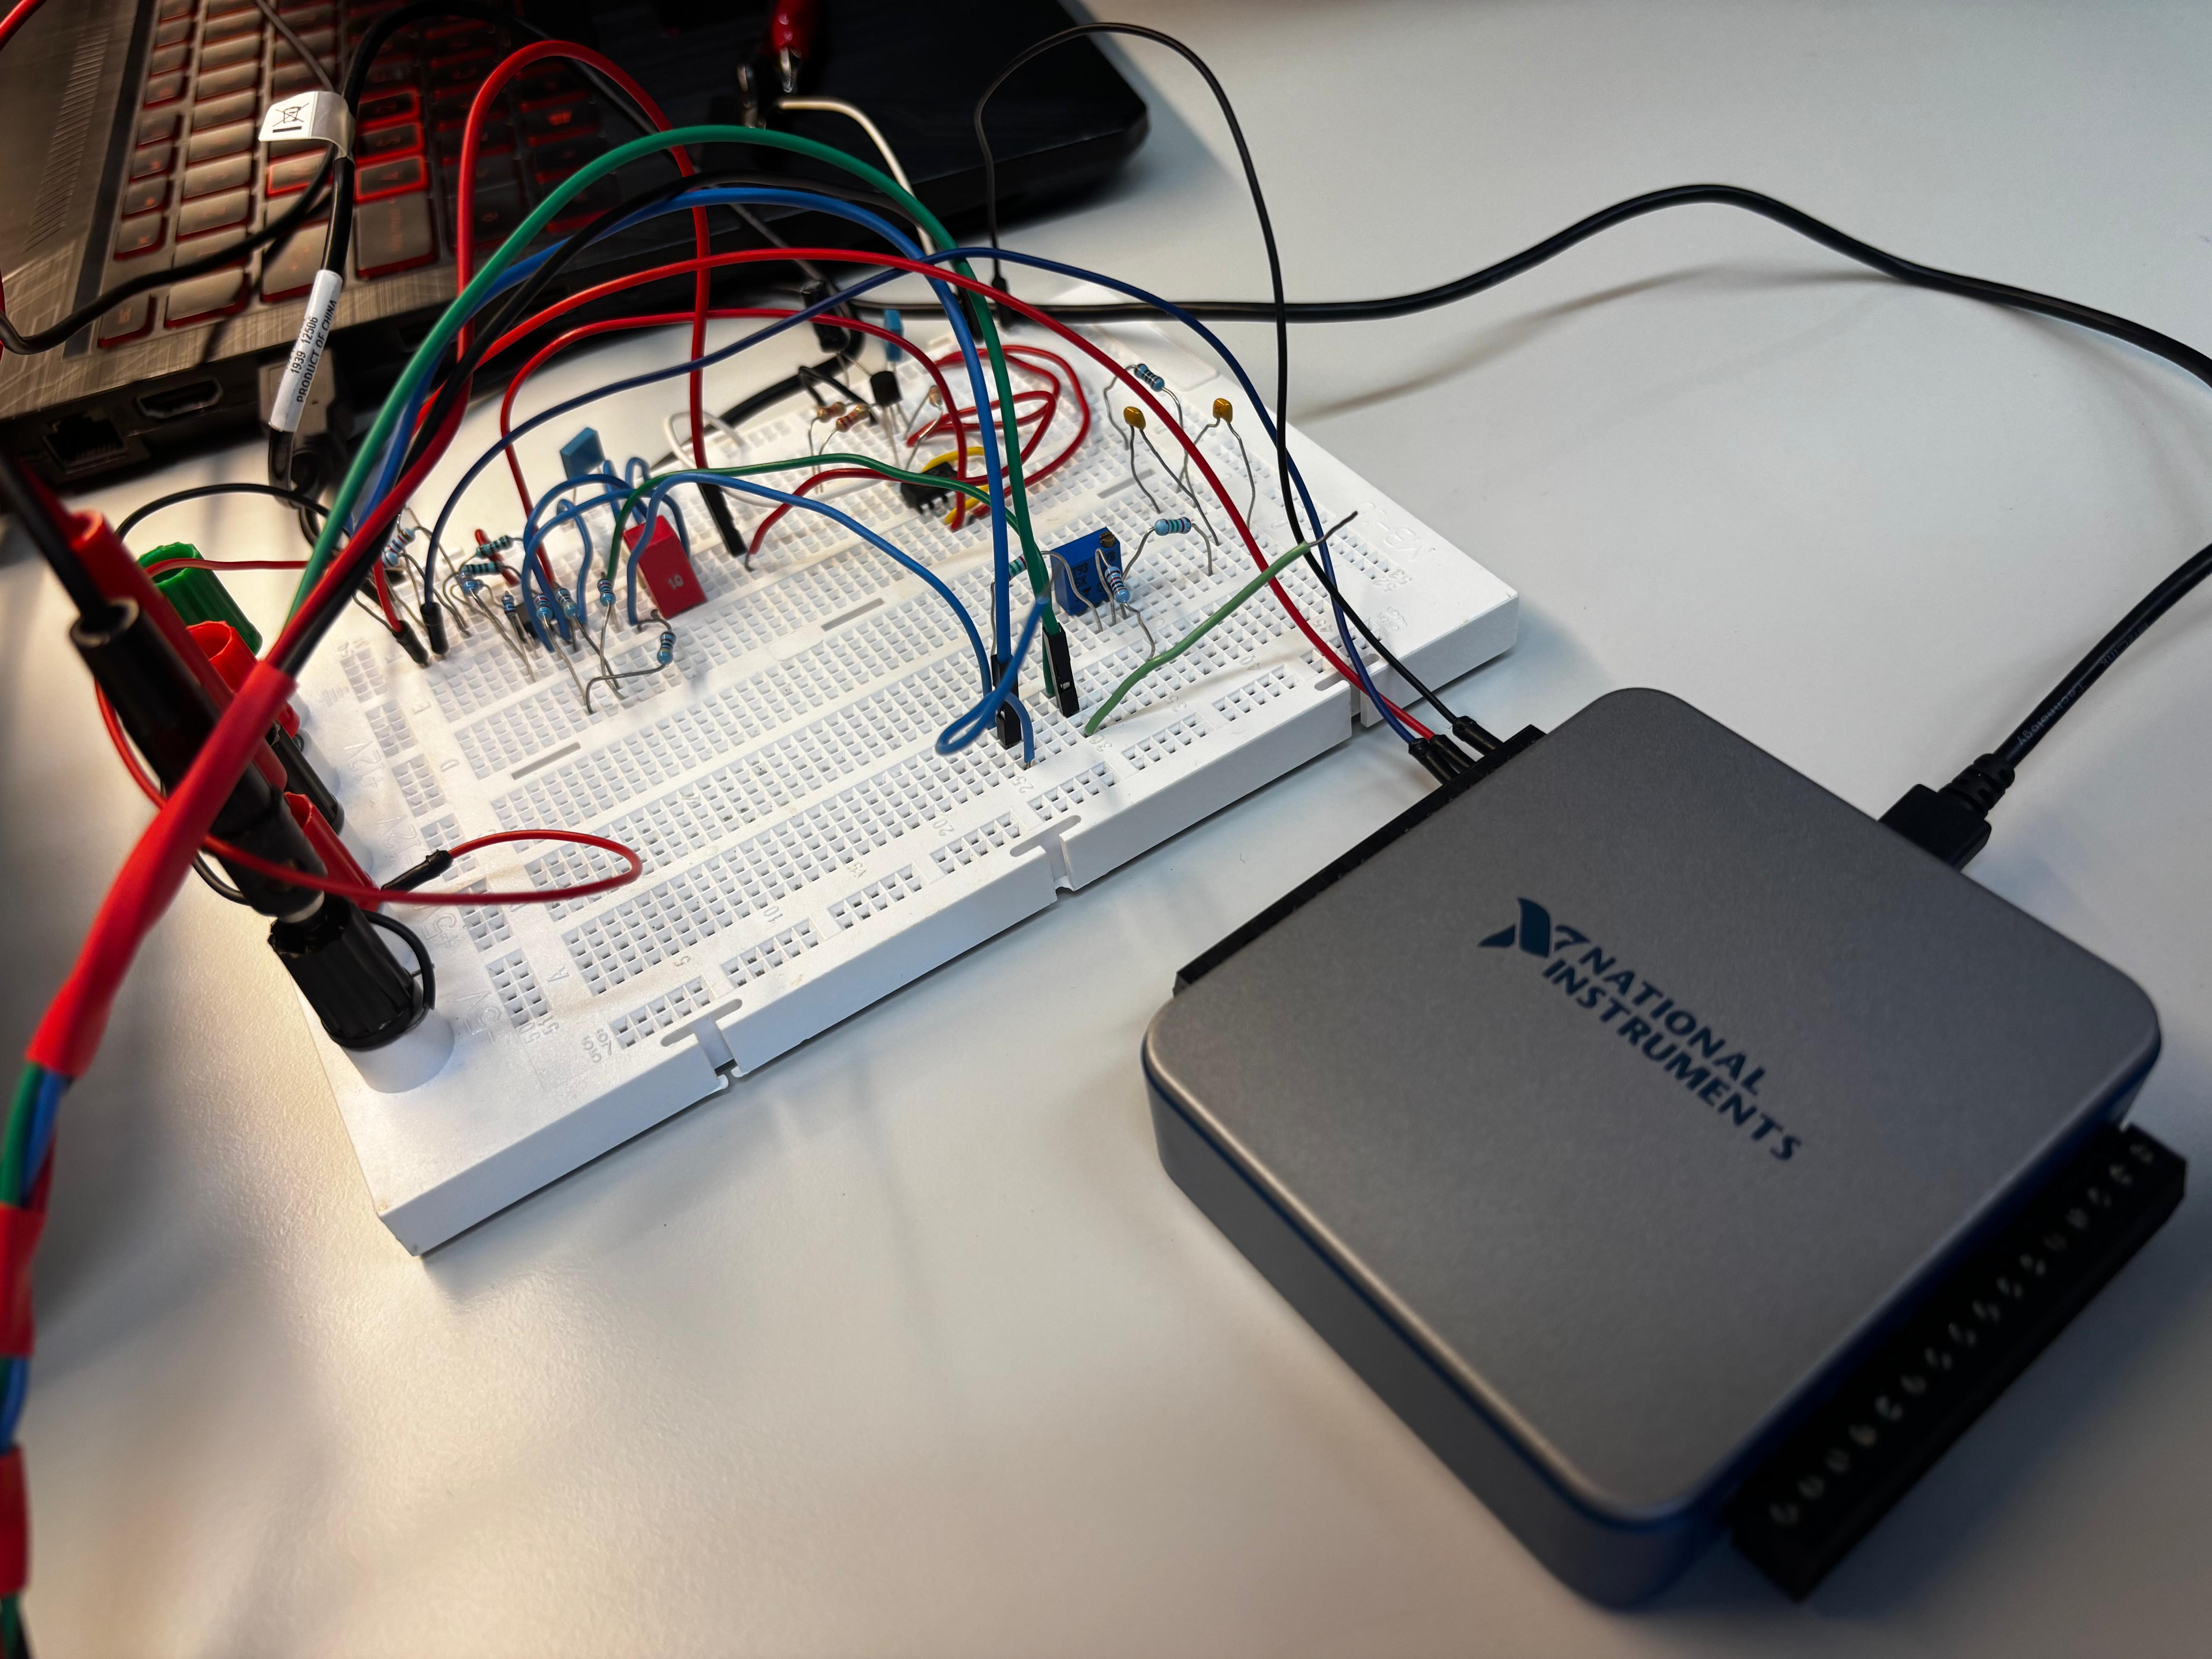
\includegraphics[width=0.65\textwidth]{figs/montaje_final.jpeg}
    \caption{Montaje final.}
    \label{fig:pedestal}
\end{figure}